\documentclass{article} % For LaTeX2e
\usepackage{iclr2022_conference,times}
% Optional math commands from https://github.com/goodfeli/dlbook_notation.
%%%%% NEW MATH DEFINITIONS %%%%%

\usepackage{amsmath,amsfonts,bm}

% Mark sections of captions for referring to divisions of figures
\newcommand{\figleft}{{\em (Left)}}
\newcommand{\figcenter}{{\em (Center)}}
\newcommand{\figright}{{\em (Right)}}
\newcommand{\figtop}{{\em (Top)}}
\newcommand{\figbottom}{{\em (Bottom)}}
\newcommand{\captiona}{{\em (a)}}
\newcommand{\captionb}{{\em (b)}}
\newcommand{\captionc}{{\em (c)}}
\newcommand{\captiond}{{\em (d)}}

% Highlight a newly defined term
\newcommand{\newterm}[1]{{\bf #1}}


% Figure reference, lower-case.
\def\figref#1{figure~\ref{#1}}
% Figure reference, capital. For start of sentence
\def\Figref#1{Figure~\ref{#1}}
\def\twofigref#1#2{figures \ref{#1} and \ref{#2}}
\def\quadfigref#1#2#3#4{figures \ref{#1}, \ref{#2}, \ref{#3} and \ref{#4}}
% Section reference, lower-case.
\def\secref#1{section~\ref{#1}}
% Section reference, capital.
\def\Secref#1{Section~\ref{#1}}
% Reference to two sections.
\def\twosecrefs#1#2{sections \ref{#1} and \ref{#2}}
% Reference to three sections.
\def\secrefs#1#2#3{sections \ref{#1}, \ref{#2} and \ref{#3}}
% Reference to an equation, lower-case.
\def\eqref#1{equation~\ref{#1}}
% Reference to an equation, upper case
\def\Eqref#1{Equation~\ref{#1}}
% A raw reference to an equation---avoid using if possible
\def\plaineqref#1{\ref{#1}}
% Reference to a chapter, lower-case.
\def\chapref#1{chapter~\ref{#1}}
% Reference to an equation, upper case.
\def\Chapref#1{Chapter~\ref{#1}}
% Reference to a range of chapters
\def\rangechapref#1#2{chapters\ref{#1}--\ref{#2}}
% Reference to an algorithm, lower-case.
\def\algref#1{algorithm~\ref{#1}}
% Reference to an algorithm, upper case.
\def\Algref#1{Algorithm~\ref{#1}}
\def\twoalgref#1#2{algorithms \ref{#1} and \ref{#2}}
\def\Twoalgref#1#2{Algorithms \ref{#1} and \ref{#2}}
% Reference to a part, lower case
\def\partref#1{part~\ref{#1}}
% Reference to a part, upper case
\def\Partref#1{Part~\ref{#1}}
\def\twopartref#1#2{parts \ref{#1} and \ref{#2}}

\def\ceil#1{\lceil #1 \rceil}
\def\floor#1{\lfloor #1 \rfloor}
\def\1{\bm{1}}
\newcommand{\train}{\mathcal{D}}
\newcommand{\valid}{\mathcal{D_{\mathrm{valid}}}}
\newcommand{\test}{\mathcal{D_{\mathrm{test}}}}

\def\eps{{\epsilon}}


% Random variables
\def\reta{{\textnormal{$\eta$}}}
\def\ra{{\textnormal{a}}}
\def\rb{{\textnormal{b}}}
\def\rc{{\textnormal{c}}}
\def\rd{{\textnormal{d}}}
\def\re{{\textnormal{e}}}
\def\rf{{\textnormal{f}}}
\def\rg{{\textnormal{g}}}
\def\rh{{\textnormal{h}}}
\def\ri{{\textnormal{i}}}
\def\rj{{\textnormal{j}}}
\def\rk{{\textnormal{k}}}
\def\rl{{\textnormal{l}}}
% rm is already a command, just don't name any random variables m
\def\rn{{\textnormal{n}}}
\def\ro{{\textnormal{o}}}
\def\rp{{\textnormal{p}}}
\def\rq{{\textnormal{q}}}
\def\rr{{\textnormal{r}}}
\def\rs{{\textnormal{s}}}
\def\rt{{\textnormal{t}}}
\def\ru{{\textnormal{u}}}
\def\rv{{\textnormal{v}}}
\def\rw{{\textnormal{w}}}
\def\rx{{\textnormal{x}}}
\def\ry{{\textnormal{y}}}
\def\rz{{\textnormal{z}}}

% Random vectors
\def\rvepsilon{{\mathbf{\epsilon}}}
\def\rvtheta{{\mathbf{\theta}}}
\def\rva{{\mathbf{a}}}
\def\rvb{{\mathbf{b}}}
\def\rvc{{\mathbf{c}}}
\def\rvd{{\mathbf{d}}}
\def\rve{{\mathbf{e}}}
\def\rvf{{\mathbf{f}}}
\def\rvg{{\mathbf{g}}}
\def\rvh{{\mathbf{h}}}
\def\rvu{{\mathbf{i}}}
\def\rvj{{\mathbf{j}}}
\def\rvk{{\mathbf{k}}}
\def\rvl{{\mathbf{l}}}
\def\rvm{{\mathbf{m}}}
\def\rvn{{\mathbf{n}}}
\def\rvo{{\mathbf{o}}}
\def\rvp{{\mathbf{p}}}
\def\rvq{{\mathbf{q}}}
\def\rvr{{\mathbf{r}}}
\def\rvs{{\mathbf{s}}}
\def\rvt{{\mathbf{t}}}
\def\rvu{{\mathbf{u}}}
\def\rvv{{\mathbf{v}}}
\def\rvw{{\mathbf{w}}}
\def\rvx{{\mathbf{x}}}
\def\rvy{{\mathbf{y}}}
\def\rvz{{\mathbf{z}}}

% Elements of random vectors
\def\erva{{\textnormal{a}}}
\def\ervb{{\textnormal{b}}}
\def\ervc{{\textnormal{c}}}
\def\ervd{{\textnormal{d}}}
\def\erve{{\textnormal{e}}}
\def\ervf{{\textnormal{f}}}
\def\ervg{{\textnormal{g}}}
\def\ervh{{\textnormal{h}}}
\def\ervi{{\textnormal{i}}}
\def\ervj{{\textnormal{j}}}
\def\ervk{{\textnormal{k}}}
\def\ervl{{\textnormal{l}}}
\def\ervm{{\textnormal{m}}}
\def\ervn{{\textnormal{n}}}
\def\ervo{{\textnormal{o}}}
\def\ervp{{\textnormal{p}}}
\def\ervq{{\textnormal{q}}}
\def\ervr{{\textnormal{r}}}
\def\ervs{{\textnormal{s}}}
\def\ervt{{\textnormal{t}}}
\def\ervu{{\textnormal{u}}}
\def\ervv{{\textnormal{v}}}
\def\ervw{{\textnormal{w}}}
\def\ervx{{\textnormal{x}}}
\def\ervy{{\textnormal{y}}}
\def\ervz{{\textnormal{z}}}

% Random matrices
\def\rmA{{\mathbf{A}}}
\def\rmB{{\mathbf{B}}}
\def\rmC{{\mathbf{C}}}
\def\rmD{{\mathbf{D}}}
\def\rmE{{\mathbf{E}}}
\def\rmF{{\mathbf{F}}}
\def\rmG{{\mathbf{G}}}
\def\rmH{{\mathbf{H}}}
\def\rmI{{\mathbf{I}}}
\def\rmJ{{\mathbf{J}}}
\def\rmK{{\mathbf{K}}}
\def\rmL{{\mathbf{L}}}
\def\rmM{{\mathbf{M}}}
\def\rmN{{\mathbf{N}}}
\def\rmO{{\mathbf{O}}}
\def\rmP{{\mathbf{P}}}
\def\rmQ{{\mathbf{Q}}}
\def\rmR{{\mathbf{R}}}
\def\rmS{{\mathbf{S}}}
\def\rmT{{\mathbf{T}}}
\def\rmU{{\mathbf{U}}}
\def\rmV{{\mathbf{V}}}
\def\rmW{{\mathbf{W}}}
\def\rmX{{\mathbf{X}}}
\def\rmY{{\mathbf{Y}}}
\def\rmZ{{\mathbf{Z}}}

% Elements of random matrices
\def\ermA{{\textnormal{A}}}
\def\ermB{{\textnormal{B}}}
\def\ermC{{\textnormal{C}}}
\def\ermD{{\textnormal{D}}}
\def\ermE{{\textnormal{E}}}
\def\ermF{{\textnormal{F}}}
\def\ermG{{\textnormal{G}}}
\def\ermH{{\textnormal{H}}}
\def\ermI{{\textnormal{I}}}
\def\ermJ{{\textnormal{J}}}
\def\ermK{{\textnormal{K}}}
\def\ermL{{\textnormal{L}}}
\def\ermM{{\textnormal{M}}}
\def\ermN{{\textnormal{N}}}
\def\ermO{{\textnormal{O}}}
\def\ermP{{\textnormal{P}}}
\def\ermQ{{\textnormal{Q}}}
\def\ermR{{\textnormal{R}}}
\def\ermS{{\textnormal{S}}}
\def\ermT{{\textnormal{T}}}
\def\ermU{{\textnormal{U}}}
\def\ermV{{\textnormal{V}}}
\def\ermW{{\textnormal{W}}}
\def\ermX{{\textnormal{X}}}
\def\ermY{{\textnormal{Y}}}
\def\ermZ{{\textnormal{Z}}}

% Vectors
\def\vzero{{\bm{0}}}
\def\vone{{\bm{1}}}
\def\vmu{{\bm{\mu}}}
\def\vtheta{{\bm{\theta}}}
\def\va{{\bm{a}}}
\def\vb{{\bm{b}}}
\def\vc{{\bm{c}}}
\def\vd{{\bm{d}}}
\def\ve{{\bm{e}}}
\def\vf{{\bm{f}}}
\def\vg{{\bm{g}}}
\def\vh{{\bm{h}}}
\def\vi{{\bm{i}}}
\def\vj{{\bm{j}}}
\def\vk{{\bm{k}}}
\def\vl{{\bm{l}}}
\def\vm{{\bm{m}}}
\def\vn{{\bm{n}}}
\def\vo{{\bm{o}}}
\def\vp{{\bm{p}}}
\def\vq{{\bm{q}}}
\def\vr{{\bm{r}}}
\def\vs{{\bm{s}}}
\def\vt{{\bm{t}}}
\def\vu{{\bm{u}}}
\def\vv{{\bm{v}}}
\def\vw{{\bm{w}}}
\def\vx{{\bm{x}}}
\def\vy{{\bm{y}}}
\def\vz{{\bm{z}}}

% Elements of vectors
\def\evalpha{{\alpha}}
\def\evbeta{{\beta}}
\def\evepsilon{{\epsilon}}
\def\evlambda{{\lambda}}
\def\evomega{{\omega}}
\def\evmu{{\mu}}
\def\evpsi{{\psi}}
\def\evsigma{{\sigma}}
\def\evtheta{{\theta}}
\def\eva{{a}}
\def\evb{{b}}
\def\evc{{c}}
\def\evd{{d}}
\def\eve{{e}}
\def\evf{{f}}
\def\evg{{g}}
\def\evh{{h}}
\def\evi{{i}}
\def\evj{{j}}
\def\evk{{k}}
\def\evl{{l}}
\def\evm{{m}}
\def\evn{{n}}
\def\evo{{o}}
\def\evp{{p}}
\def\evq{{q}}
\def\evr{{r}}
\def\evs{{s}}
\def\evt{{t}}
\def\evu{{u}}
\def\evv{{v}}
\def\evw{{w}}
\def\evx{{x}}
\def\evy{{y}}
\def\evz{{z}}

% Matrix
\def\mA{{\bm{A}}}
\def\mB{{\bm{B}}}
\def\mC{{\bm{C}}}
\def\mD{{\bm{D}}}
\def\mE{{\bm{E}}}
\def\mF{{\bm{F}}}
\def\mG{{\bm{G}}}
\def\mH{{\bm{H}}}
\def\mI{{\bm{I}}}
\def\mJ{{\bm{J}}}
\def\mK{{\bm{K}}}
\def\mL{{\bm{L}}}
\def\mM{{\bm{M}}}
\def\mN{{\bm{N}}}
\def\mO{{\bm{O}}}
\def\mP{{\bm{P}}}
\def\mQ{{\bm{Q}}}
\def\mR{{\bm{R}}}
\def\mS{{\bm{S}}}
\def\mT{{\bm{T}}}
\def\mU{{\bm{U}}}
\def\mV{{\bm{V}}}
\def\mW{{\bm{W}}}
\def\mX{{\bm{X}}}
\def\mY{{\bm{Y}}}
\def\mZ{{\bm{Z}}}
\def\mBeta{{\bm{\beta}}}
\def\mPhi{{\bm{\Phi}}}
\def\mLambda{{\bm{\Lambda}}}
\def\mSigma{{\bm{\Sigma}}}

% Tensor
\DeclareMathAlphabet{\mathsfit}{\encodingdefault}{\sfdefault}{m}{sl}
\SetMathAlphabet{\mathsfit}{bold}{\encodingdefault}{\sfdefault}{bx}{n}
\newcommand{\tens}[1]{\bm{\mathsfit{#1}}}
\def\tA{{\tens{A}}}
\def\tB{{\tens{B}}}
\def\tC{{\tens{C}}}
\def\tD{{\tens{D}}}
\def\tE{{\tens{E}}}
\def\tF{{\tens{F}}}
\def\tG{{\tens{G}}}
\def\tH{{\tens{H}}}
\def\tI{{\tens{I}}}
\def\tJ{{\tens{J}}}
\def\tK{{\tens{K}}}
\def\tL{{\tens{L}}}
\def\tM{{\tens{M}}}
\def\tN{{\tens{N}}}
\def\tO{{\tens{O}}}
\def\tP{{\tens{P}}}
\def\tQ{{\tens{Q}}}
\def\tR{{\tens{R}}}
\def\tS{{\tens{S}}}
\def\tT{{\tens{T}}}
\def\tU{{\tens{U}}}
\def\tV{{\tens{V}}}
\def\tW{{\tens{W}}}
\def\tX{{\tens{X}}}
\def\tY{{\tens{Y}}}
\def\tZ{{\tens{Z}}}


% Graph
\def\gA{{\mathcal{A}}}
\def\gB{{\mathcal{B}}}
\def\gC{{\mathcal{C}}}
\def\gD{{\mathcal{D}}}
\def\gE{{\mathcal{E}}}
\def\gF{{\mathcal{F}}}
\def\gG{{\mathcal{G}}}
\def\gH{{\mathcal{H}}}
\def\gI{{\mathcal{I}}}
\def\gJ{{\mathcal{J}}}
\def\gK{{\mathcal{K}}}
\def\gL{{\mathcal{L}}}
\def\gM{{\mathcal{M}}}
\def\gN{{\mathcal{N}}}
\def\gO{{\mathcal{O}}}
\def\gP{{\mathcal{P}}}
\def\gQ{{\mathcal{Q}}}
\def\gR{{\mathcal{R}}}
\def\gS{{\mathcal{S}}}
\def\gT{{\mathcal{T}}}
\def\gU{{\mathcal{U}}}
\def\gV{{\mathcal{V}}}
\def\gW{{\mathcal{W}}}
\def\gX{{\mathcal{X}}}
\def\gY{{\mathcal{Y}}}
\def\gZ{{\mathcal{Z}}}

% Sets
\def\sA{{\mathbb{A}}}
\def\sB{{\mathbb{B}}}
\def\sC{{\mathbb{C}}}
\def\sD{{\mathbb{D}}}
% Don't use a set called E, because this would be the same as our symbol
% for expectation.
\def\sF{{\mathbb{F}}}
\def\sG{{\mathbb{G}}}
\def\sH{{\mathbb{H}}}
\def\sI{{\mathbb{I}}}
\def\sJ{{\mathbb{J}}}
\def\sK{{\mathbb{K}}}
\def\sL{{\mathbb{L}}}
\def\sM{{\mathbb{M}}}
\def\sN{{\mathbb{N}}}
\def\sO{{\mathbb{O}}}
\def\sP{{\mathbb{P}}}
\def\sQ{{\mathbb{Q}}}
\def\sR{{\mathbb{R}}}
\def\sS{{\mathbb{S}}}
\def\sT{{\mathbb{T}}}
\def\sU{{\mathbb{U}}}
\def\sV{{\mathbb{V}}}
\def\sW{{\mathbb{W}}}
\def\sX{{\mathbb{X}}}
\def\sY{{\mathbb{Y}}}
\def\sZ{{\mathbb{Z}}}

% Entries of a matrix
\def\emLambda{{\Lambda}}
\def\emA{{A}}
\def\emB{{B}}
\def\emC{{C}}
\def\emD{{D}}
\def\emE{{E}}
\def\emF{{F}}
\def\emG{{G}}
\def\emH{{H}}
\def\emI{{I}}
\def\emJ{{J}}
\def\emK{{K}}
\def\emL{{L}}
\def\emM{{M}}
\def\emN{{N}}
\def\emO{{O}}
\def\emP{{P}}
\def\emQ{{Q}}
\def\emR{{R}}
\def\emS{{S}}
\def\emT{{T}}
\def\emU{{U}}
\def\emV{{V}}
\def\emW{{W}}
\def\emX{{X}}
\def\emY{{Y}}
\def\emZ{{Z}}
\def\emSigma{{\Sigma}}

% entries of a tensor
% Same font as tensor, without \bm wrapper
\newcommand{\etens}[1]{\mathsfit{#1}}
\def\etLambda{{\etens{\Lambda}}}
\def\etA{{\etens{A}}}
\def\etB{{\etens{B}}}
\def\etC{{\etens{C}}}
\def\etD{{\etens{D}}}
\def\etE{{\etens{E}}}
\def\etF{{\etens{F}}}
\def\etG{{\etens{G}}}
\def\etH{{\etens{H}}}
\def\etI{{\etens{I}}}
\def\etJ{{\etens{J}}}
\def\etK{{\etens{K}}}
\def\etL{{\etens{L}}}
\def\etM{{\etens{M}}}
\def\etN{{\etens{N}}}
\def\etO{{\etens{O}}}
\def\etP{{\etens{P}}}
\def\etQ{{\etens{Q}}}
\def\etR{{\etens{R}}}
\def\etS{{\etens{S}}}
\def\etT{{\etens{T}}}
\def\etU{{\etens{U}}}
\def\etV{{\etens{V}}}
\def\etW{{\etens{W}}}
\def\etX{{\etens{X}}}
\def\etY{{\etens{Y}}}
\def\etZ{{\etens{Z}}}

% The true underlying data generating distribution
\newcommand{\pdata}{p_{\rm{data}}}
% The empirical distribution defined by the training set
\newcommand{\ptrain}{\hat{p}_{\rm{data}}}
\newcommand{\Ptrain}{\hat{P}_{\rm{data}}}
% The model distribution
\newcommand{\pmodel}{p_{\rm{model}}}
\newcommand{\Pmodel}{P_{\rm{model}}}
\newcommand{\ptildemodel}{\tilde{p}_{\rm{model}}}
% Stochastic autoencoder distributions
\newcommand{\pencode}{p_{\rm{encoder}}}
\newcommand{\pdecode}{p_{\rm{decoder}}}
\newcommand{\precons}{p_{\rm{reconstruct}}}

\newcommand{\laplace}{\mathrm{Laplace}} % Laplace distribution

\newcommand{\E}{\mathbb{E}}
\newcommand{\Ls}{\mathcal{L}}
\newcommand{\R}{\mathbb{R}}
\newcommand{\emp}{\tilde{p}}
\newcommand{\lr}{\alpha}
\newcommand{\reg}{\lambda}
\newcommand{\rect}{\mathrm{rectifier}}
\newcommand{\softmax}{\mathrm{softmax}}
\newcommand{\sigmoid}{\sigma}
\newcommand{\softplus}{\zeta}
\newcommand{\KL}{D_{\mathrm{KL}}}
\newcommand{\Var}{\mathrm{Var}}
\newcommand{\standarderror}{\mathrm{SE}}
\newcommand{\Cov}{\mathrm{Cov}}
% Wolfram Mathworld says $L^2$ is for function spaces and $\ell^2$ is for vectors
% But then they seem to use $L^2$ for vectors throughout the site, and so does
% wikipedia.
\newcommand{\normlzero}{L^0}
\newcommand{\normlone}{L^1}
\newcommand{\normltwo}{L^2}
\newcommand{\normlp}{L^p}
\newcommand{\normmax}{L^\infty}

\newcommand{\parents}{Pa} % See usage in notation.tex. Chosen to match Daphne's book.

\DeclareMathOperator*{\argmax}{arg\,max}
\DeclareMathOperator*{\argmin}{arg\,min}

\DeclareMathOperator{\sign}{sign}
\DeclareMathOperator{\Tr}{Tr}
\let\ab\allowbreak


%######## APS360: Uncomment your submission name
\newcommand{\apsname}{Project Proposal}
%\newcommand{\apsname}{Progress Report}
%\newcommand{\apsname}{Final Report}

%######## APS360: Put your Group Number here
\newcommand{\gpnumber}{11}

\usepackage{hyperref}
\usepackage{url}
\usepackage{graphicx}
\usepackage{enumitem}
\usepackage{tabularx}
\usepackage{float}

%######## APS360: Put your project Title here
\title{AI Writing Detector: A Deep Learning Approach to Distinguish Human and AI-Generated Text}
 
%######## APS360: Put your names, student IDs and Emails here
\author{Zahra Mohamed Suhail  \\
Student\# 1008997016 \\
\texttt{zahra.suhail@mail.utoronto.ca} \\
\And
Tajrian Islam \\
Student\# 1007939251 \\
\texttt{tajriansyeda.islam@mail.utoronto.ca} \\
\And
Xin Ling (Grace) Li  \\
Student\# 1010143113 \\
\texttt{xlgrace.li@mail.utoronto.ca} \\
\And
Sophia Hill  \\
Student\# 1007865883 \\
\texttt{sophia.hill@mail.utoronto.ca} \\
\And
}

\newcommand{\fix}{\marginpar{FIX}}
\newcommand{\new}{\marginpar{NEW}}

\iclrfinalcopy 
\begin{document}

\maketitle
\newpage

\section{Introduction}
With the introduction of ChatGPT in 2022, generative Artificial Intelligence (AI) has become widely accessible, particularly to generate written content at a level similar to that created by humans. However, this quickly raised ethical concerns, as people have begun to pass off AI-written content as their own, which has created issues of plagiarism in educational, professional, and creative spaces. Thus, a need has arisen for a deep learning algorithm that can efficiently and accurately detect AI-written content to mitigate the implications to academic, professional, and artistic integrity, and to prevent inaccurate accusations of plagiarism. Therefore, we propose to create an AI Writing Detector that can accurately detect the complexities of human-written, AI-written, and mixed content. AI algorithms used to generate written content have detectable structures that differ from that of humans. Through a Multi-Layer Perceptron (MLP) model, our team will create an AI Writing Detector that will help resolve the issues of integrity and of the authorship in the age of AI.

\section{Illustration}
Our AI Writing Detector's overall pipeline consists of text preprocessing, feature extractions, and a MLP neural network to classify between AI-generated and human-written text. An illustration of our proposed AI Writing Detector Pipeline is shown in Figure 1.

\begin{figure}[htbp]
    \centering
    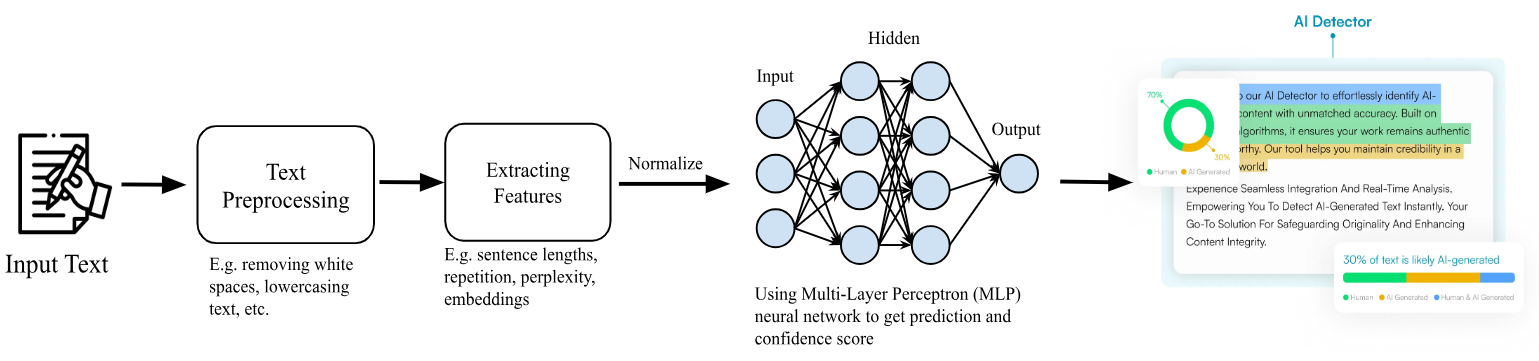
\includegraphics[width=0.9\linewidth]{illustration.png}
    \caption{An illustration of our proposed AI Writing Detector Pipeline is shown} \citep{Freepik}
    \label{fig:pipeline}
\end{figure}

\section{Background \& Related Work}

\subsection{Related Papers}

\textbf{``Detecting Generative Artificial Intelligence Essays using Large Language Models: Machine and Deep Learning Approaches''}

This study analyses the efficacy of different deep learning models to identify human written and AI written essays. The algorithms it discusses are logistic regression, Support Vector Machine (SVM), decision trees, random forests, K-Nearest Neighbours (KNN), and Long Short Term Memory (LSTM). The research used Term Frequency-Inverse Document Frequency (TF-IDF) to prepare their data. It found that SVM and LSTM were the most accurate algorithms, though LSTM is more demanding computationally.

\textbf{``Deep learning detection method for large language models-generated scientific content''}

This paper outlines a model called AI-Catcher developed to identify AI generated writing, citations, and data in scientific papers, treated as a binary classification problem. AI-Catcher uses two models to identify human versus AI generated text: the MLP and a Convolutional Neural Network (CNN). For the MLP, it prepares the data through text cleaning, text encoding, and padding. The MLP model then has five hidden layers, each with 256 neurons, where each layer applies a linear transformation and then ReLU activation. For the CNN model, it prepares the data through extraction of thirteen linguistic and statistical features from the text. Then, it uses the embedding layer to put the encoded integers into vectors, followed by a dropout layer, and then a convolutional layer connected to a global max pooling layer. The results of the two are then concatenated into a single feature vector, which goes through two additional hidden layers. The accuracy, precision, recall, and F1 score of the model were assessed based on confusion matrices. This research was only conducted using scientific papers written by humans or generated by ChatGPT (as opposed to other LLMs).

\textbf{``Detecting AI-generated essays: the ChatGPT challenge''}

This research paper from early 2023 investigates effective algorithms to identify human and ChatGPT generated essays. They used a n-gram bag-of-words (BOW) language model for the classifier input with n=5. They tested the performance of Support Vector Machine, Naïve Bayes, Logistic Regression, Random Forest, and Neural Network classification algorithms and then tested the performance of an Ensemble Learning (EL) classifier with the five algorithms fed to it. The findings stated that their SVM, which was modified to eliminate False Negatives entirely, was the most efficient algorithm. The study emphasized eliminating False Negatives (human written essays labelled as AI) due to the ethical implications of incorrectly blaming students for plagiarism with ChatGPT. SVM alone had a slightly lower accuracy than EL, but had better recall and F2 scores. Their SVM model also had fewer False Negatives than OpenAI Detector, GPTZero, and Copyleaks on test data and a 100\% accuracy in detecting human-written essays, despite a lower overall accuracy. This research did also have a relatively small sample size, with 230 total essays for training and 150 for testing (Cingillioglu, 2023).

\subsection{Current Software Solutions}

\textbf{GPTZero} ~\citep{GPTZero}

GPTZero is an AI detector that scans for AI generated writing on a sentence, paragraph, and document level. It can detect AI written content generated by ChatGPT, GPT-4, GPT-3, GPT-2, LLaMA, and derivatives of those models. It claims to have a 99\% accuracy and has an extension that can be added to Google Classroom and Google Docs. It can also identify if a text is entirely human written, entirely AI written, or mixed. However some of its features are locked behind a paid subscription, such as its ability to indicate the most human or AI written parts of a sample of writing and the number of characters, words, or files that can be submitted to it at a time, and it is also primarily for the analysis of English text.

\textbf{Copyleaks} \citep{Copyleaks}

Copyleaks is a plagiarism detector and AI detector. It works with 30+ languages and claims to have a 99.8\% accuracy and a 0.2\% false positive rate. It can detect text written by LLMs like ChatGPT, Gemini, DeepSeek, Claude, Jasper 3, LLaMA, and T5. It also shows the percentage of AI in a piece of text and can account for different detection sensitivity levels. It claims to have the capability to identify plagiarism and paraphrasing done with AI and that it can identify human written, AI written, and mixed text. It has a minimum requirement for the number of characters (350) to accurately determine the presence of AI. Copyleaks also has Google Docs extension and mostly requires a paid subscription, with only a limited number of free uses.

\textbf{Grammarly} ~\citep{Grammarly}

Grammarly, an AI based grammar checker, also has its own AI detector. It can detect writing generated by Grammarly, ChatGPT, Google Gemini, and Claude, and it can show the percentage of text that is AI generated. However, it is only available with certain paid subscriptions and they have not stated the accuracy rate of their checker.

\newpage
\section{Data Processing}
Figure 2 illustrates the data process pipeline. It demonstrates the effort to source, repurpose, clean, and structure data rather than just using a pre-existing dataset.

\begin{figure}[H]
    \centering
    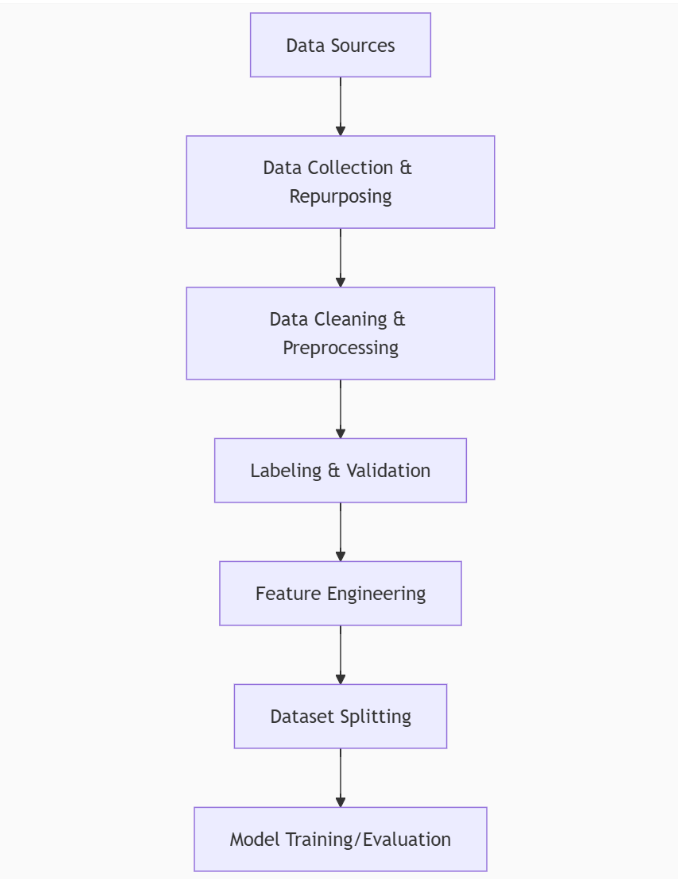
\includegraphics[width=0.7\linewidth,height=0.4\textheight,keepaspectratio]{data.png}
    \caption{Schematic overview of the proposed data processing methodology}
    \label{fig:pipeline}
\end{figure}

\subsection{Data Sources}
To ensure a robust and diverse dataset, we will undertake an extensive data collection and processing effort, prioritizing originality and rigor over the use of pre-existing datasets. Our data is sourced from multiple origins to enhance generalization:

\begin{itemize}
    \item \textbf{Human-Written Text:}
    \begin{itemize}
        \item \textbf{Academic Papers \& Essays:}
        \begin{itemize}
            \item Sources: arXiv, PubMed, OpenAlex (for older literature)
            \item Why: High-quality, structured, and varied writing styles
        \end{itemize}
        
        \item \textbf{News Articles:}
        \begin{itemize}
            \item Sources: CBC News, BBC News, Reuters
            \item Why: Factual, professionally edited, diverse topics
        \end{itemize}
        
        \item \textbf{Creative Writing:}
        \begin{itemize}
            \item Sources: Wattpad, Fanfiction.net, literary blogs
            \item Why: Informal, narrative-driven, varied author styles
        \end{itemize}
        
        \item \textbf{Social Media \& Forums:}
        \begin{itemize}
            \item Sources: Reddit (long-form posts), Quora, Facebook
            \item Why: Conversational, personal, and opinionated writing
        \end{itemize}
    \end{itemize}
    
    \item \textbf{AI-Generated Text:}
    \begin{itemize}
        \item GPT Models (OpenAI, Gemini, Deepseek):
        \begin{itemize}
            \item Using the API calls, one can generate synthetic text with varying prompts (e.g., essays, stories, technical writing)
            \item Use different model versions (GPT-3.5, GPT-4, etc.) to capture evolution
        \end{itemize}

         \item Kaggle:
        \begin{itemize}
            \item Provides various styles of texts that one can compare, for example one can fetch a dataset that contains generated texts from LLM.
        \end{itemize}
    \end{itemize}
    
    \item \textbf{Hybrid (Human + AI Edited):}
    \begin{itemize}
        \item Wikipedia Edits:
        \begin{itemize}
            \item By using the edit history one can compare pre- and post-GPT-4 Wikipedia edits
        \end{itemize}
        
        \item GitHub Docs:
        \begin{itemize}
            \item Some repositories use AI for README generation, this can be identified via commit logs
        \end{itemize}
    \end{itemize}
\end{itemize}

\subsection{Data Collection \& Repurposing Efforts}
We gathered data in several careful ways to make sure it was both useful and ethical:

\begin{itemize}
    \item \textbf{Web Scraping (Respectful \& Legal):}
    \begin{itemize}
        \item By using open source frameworks that can help with extracting data in an efficient manner such that delays of overloading servers are avoided, use: \textit{scrapy} or \textit{BeautifulSoup}
        \item Web scraping is legal so long as the data is publicly available
    \end{itemize}
    
    \item \textbf{Using APIs to Generate Synthetic Data:}
    \begin{itemize}
        \item OpenAI API with varied prompts (i.e "Write an essay about AI").
    \end{itemize}
    
    \item \textbf{Data Augmentation:}
    \begin{itemize}
        \item Paraphrase human text using AI to create "AI-like" samples
    \end{itemize}
    
    \item \textbf{Partnerships:}
    \begin{itemize}
        \item Collaborate with universities for student-written vs. AI-assisted essays
    \end{itemize}
\end{itemize}

\subsection{Data Cleaning \& Preprocessing}
Before using the data, we must clean and organize it to ensure quality and fairness. First, we removed duplicate or nearly identical content to avoid repetition:
\begin{itemize}
    \item \textbf{Deduplication \& Noise Removal:}
    \begin{itemize}
        \item Near-Deduplication:
        \begin{itemize}
            \item Use MinHash/LSH (Locality-Sensitive Hashing) to remove near-identical samples
        \end{itemize}
        
        \item Language Filtering:
        \begin{itemize}
            \item Keep only English text (fastText language detection, developed by Facebook AI Researchers).
        \end{itemize}
        
        \item Quality Filtering:
        \begin{itemize}
            \item Remove low-quality text (e.g., incomplete sentences, excessive repetition)
        \end{itemize}
    \end{itemize}
    
    \item \textbf{Text Normalization:}
    \begin{itemize}
        \item Lowercasing (optional, case-sensitive models may retain it)
        \item Remove boilerplate (HTML tags, ads, headers/footers)
        \item Expand contractions ("can't" $\rightarrow$ "cannot") for consistency
    \end{itemize}
    
    \item \textbf{Balancing \& Stratification:}
    \begin{itemize}
        \item Ensure balanced classes (human vs. AI) across various domains of writing (academic, creative, etc.)
    \end{itemize}
\end{itemize}

\subsection{Labeling \& Validation}
There needs to be a way in which human verification is used for labeling and validating the data.

\begin{itemize}
    \item \textbf{Human Verification:}
    \begin{itemize}
        \item Crowdsource (Amazon Mechanical Turk) to label ambiguous cases
        \item Expert review for disputed samples (e.g., linguistics PhDs)
    \end{itemize}
    
    \item \textbf{Confidence Scoring:}
    \begin{itemize}
        \item Use models (RoBERTa, GPT-detectors) to flag uncertain samples for rechecking
    \end{itemize}

    \item \textbf{Kaggle:}
    \begin{itemize}
        \item By using a dataset of LLM generated texts, provided from this source one can compare and contrast when validating data.
    \end{itemize}
\end{itemize}

\subsection{Feature Engineering}
\begin{itemize}
    \item \textbf{Stylometric Features:}
    \begin{itemize}
        \item Sentence length variance, word rarity, POS tag ratios
    \end{itemize}
    
    \item \textbf{Perplexity Scores:}
    \begin{itemize}
        \item Compare human vs. AI text using small GPT-2
    \end{itemize}
    
    \item \textbf{Watermarking Detection:}
    \begin{itemize}
        \item If watermarks are presented in the AI text(e.g., OpenAI's), incorporate detection.
    \end{itemize}
\end{itemize}

\subsection{Dataset Splitting}
\begin{itemize}
    \item Split data into: Train (70\%) / Validation (15\%) / Test (15\%)
    \item Ensure each split has no overlapping sources/authors.
    \item If testing newer AI Models. One can split based on time (e.g., train on GPT-3, test on GPT-4).
\end{itemize}

\section{Architecture}
The MLP stands out as the most effective neural network architecture for AI text detection. Studies comparing various machine learning models have shown that MLPs strike the best balance between accuracy, efficiency, and flexibility. While SVMs require manual feature engineering and LSTM networks are computationally intensive, MLPs deliver high accuracy without these drawbacks. As highlighted in the AI-Catcher study, MLPs outperform CNNs in capturing the overall coherence of text, which is a key factor in detecting AI-generated content. Unlike complex ensemble methods, which added little value in challenges like ChatGPT detection, MLPs offer a simpler, more interpretable solution that scales well. MLPs further enhance their practicality by working with both engineered features and raw text embeddings. Altogether, MLPs combine performance, simplicity, and real-world validation, making them an ideal choice for reliable, production-ready AI text detection system.

\section{Baseline Model}
Most of the research that investigates effective AI writing detection algorithms found that SVM was the best model for accuracy ~\citep{AIessays2023}, \citep{Approaches}.
Sklearn has a built-in SVM model package that can be built given specific parameters and trained on the data~\citep{GeeksForGeeks}. This would require hyperparameter tuning of the model, which would initially be based off of what was found to be effective in the literature. A 2024 study focused on the detection of human-written and AI-written texts found the default settings of Sklearn's SVM model were sufficient in training (Tariq et al., 2024). With the default settings, the kernel will be "rbf" (Radial Basis Function) for non-linear classification, the regularization parameter will be set to 1.0, and the gamma parameter set to "scale"~\citep{Approaches}.

\section{Ethical Considerations}
When creating an AI detection tool, there are many ethical concerns such as accuracy, bias, and privacy.
While we aim to make a model as accurate as possible, there is still a chance for human writing to be detected as AI. Bias in the model is another issue, which can occur from the training data. A group particularly affected by AI detection systems is that of non-native English speakers, whose writing is flagged as AI-generated more often than that of native speakers due to differences in writing styles and levels of sophistication ~\citep{stanford}. Also, the risk of a biased model is that individuals begin to fear being flagged, even without AI usage. Such fears can stop people from openly expressing themselves and limit creativity. Another ethical consideration is that many individuals may not be comfortable in having their work used for model training, and the use of their data without consent would be a breach of privacy. 
We need to be careful in training our AI model as there are a lot of consequences of false detection of AI generated writing since plagiarism is tied into a person’s credibility. With a larger dataset and the ability to learn from a variety of different texts, the team will aim to train the model to be as accurate as possible and reduce its bias.

\section{Project Plan}
We will hold weekly meetings on Mondays to discuss current progress and future steps. All forms of communications will take place online via Discord, unless specified otherwise. To ensure we do not overwrite each other's code, each member will create and work on their own branches through the use of version control. Each member will open a pull request when they wish to merge with the main branch after code reviews have been completed. 

A summary of the Project Plan timeline with assignees and deadlines is shown in Figure 3. 
\begin{figure}[htbp]
    \centering
    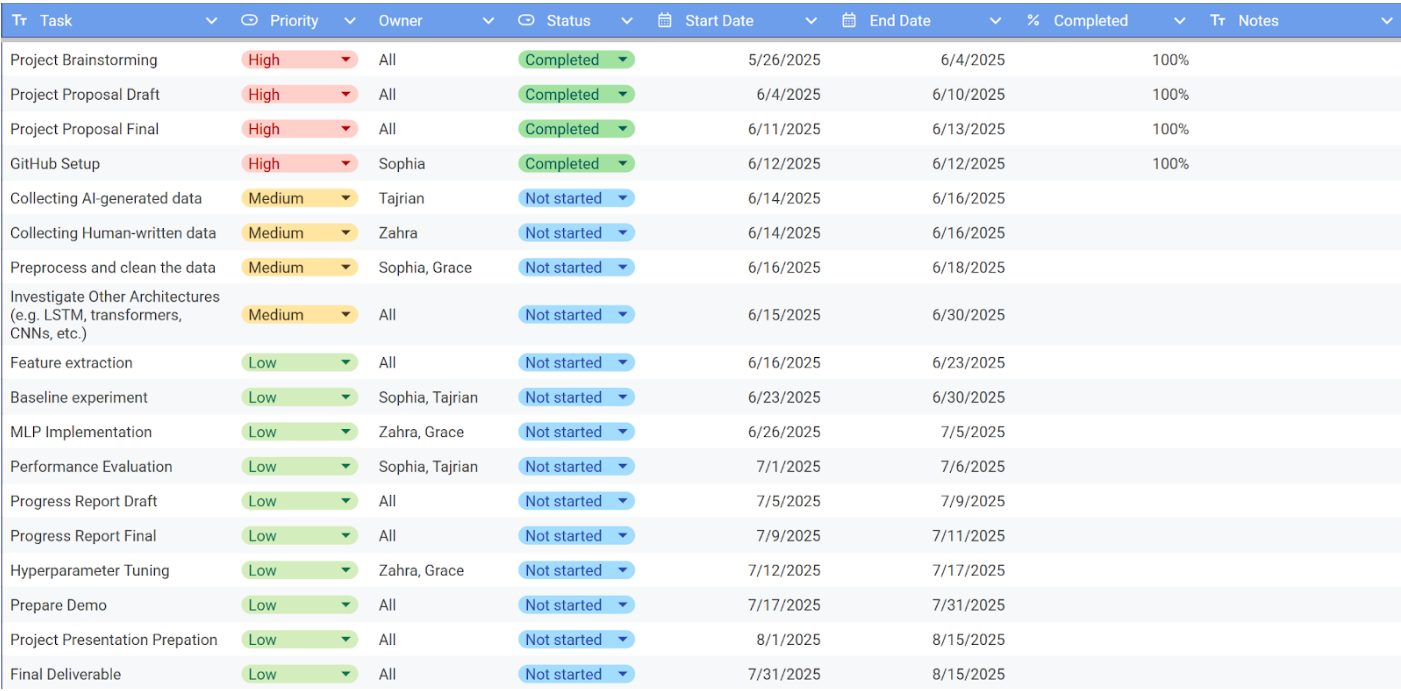
\includegraphics[width=0.9\linewidth,height=0.9\textheight,keepaspectratio]{gnatt.png}
    \caption{Project Gantt Chart}
    \label{fig:pipeline}
\end{figure}

\section{Risk Register}
In the creation of an AI model to detect if written work is made by AI, there are many problems that the team may encounter. Despite the chance of these challenges occurring, we have planned ahead on how to handle them.

\subsection{High Risk — Long Training Time Due to Large Dataset}
\textbf{Risk:} Since our dataset has a large dataset, each with at least 350 words entered at a time, training the model on the full set is likely to take a significant amount of time.\\
\textbf{Solution:} To mitigate the risk of not completing the training on time, we intend to reduce our sample size accordingly, potentially by half, ensuring that our set is still diverse. If time allows later on, we can expand the dataset for further training. 

\subsection{Medium Risk — Breach of User Privacy}
\textbf{Risk:} Since our model will be trained on written content, there is a chance that users may not want their own work to be used, making the likelihood of invading user privacy medium risk.\\
\textbf{Solution:} To mitigate any breach of privacy, we will warn users of how their data is being used. That way, whoever uses the model is giving their consent for their work to be used for training purposes and they are aware of how the data they are giving is being handled.

\subsection{Medium Risk — Detecting Human Writing as AI in Plagiarism Detection}
\textbf{Risk:} As the model is limited to the training of our dataset, the likelihood that it becomes biased and can mistake human writing as AI is a medium risk. \\
\textbf{Solution:} To mitigate the chance of the model mistaking human writing as AI, we have a large dataset with a variety of writing, teaching the model as best as possible in detecting if the written work was done by AI. This way, the model can learn from a more complex dataset and be better prepared in differentiating AI-written work from human-written work.

\subsection{Medium Risk — Missing Deadlines}
\textbf{Risk:} Our members have busy schedules with many of us working or having other activities to take care of, making the likelihood of missing deadlines a medium risk. \\
\textbf{Solution:} To mitigate the chance of missing major deadlines for the project or procrastination, the team will break tasks up and create internal deadlines using gantt charts. That way if any team member is unable to complete their part on time, there is still time for other members to help them and meet the major deadline.

\subsection{Low Risk — Team Members Dropping the Course}
\textbf{Risk:} As all of our team members need this course for our degrees, the likelihood of anyone dropping out is low risk. \\
\textbf{Solution:} To mitigate the damage to the project timeline if a team member were to drop, the team member that is leaving must notify the group as soon as possible. The team member leaving should ensure others understand the next steps of any incomplete work. Also having gantt charts and weekly meetings will help the other members redistribute responsibilities.

\hypersetup{
    colorlinks=true,
    linkcolor=blue,
    urlcolor=blue
}

\section{Link to Github/Colab}
\noindent
\href{https://github.com/shill7/APS360_Project}{\underline{\textcolor{blue}{GitHub Repository}}}

\label{last_page}

\bibliography{APS360_ref}
\bibliographystyle{iclr2022_conference}

\end{document}